\documentclass[mathserif]{beamer} 
\usepackage{eulervm} %красивый математический шрифт - по желанию
\usepackage{ulem} %зачёркивания
\usepackage{bm} %особо жирный математический
\usepackage{schemata} %для красивых блочных переходов, пользуюсь редко
\usepackage{mathtools} %улучшенная работа с типографией в math mode
\setbeamertemplate{navigation symbols}{} %отключает управляющие символы в правом нижнем углу
\usefonttheme{professionalfonts}
\usepackage{cmap} %чтобы были работающие гиперссылки
\usepackage{makeidx,fancybox,tikz}
\usetikzlibrary{automata, positioning, arrows,patterns}
\usetikzlibrary{arrows.meta}
\usepackage{tempora} %по желанию -- русские штрифты с засечками

\mode<presentation>
{
% \usetheme{Warsaw}
%  \usetheme{Frankfurt}
%  \usetheme{Singapore}
%  \usetheme{Boadilla}
%  \usetheme{Montpellier}
%  \usetheme{Szeged}
  \usetheme{CambridgeUS} %тут решайте сами, что выбрать
    % or ...

%  \usecolortheme{dolphin}
  \usecolortheme{dove} %аналогично
%  \usecolortheme{wolverine}
%  \usecolortheme{crane}

%  \usefonttheme{structurebold}
%  \usefonttheme{structuresmallcapsserif}

%  \setbeamercovered{transparent}
}
\usepackage[T1,T2A]{fontenc}
\usepackage[utf8]{inputenc}
\usepackage[english,russian]{babel}
\usepackage{amsmath,mathrsfs} %ещё больше математических символов
\usepackage{amstext}
\usepackage{graphicx,relsize}
\graphicspath{ {./../images/} }

\usepackage{color}
\definecolor{gray}{rgb}{0.4,.4,0.4} %здесь можно определить собственные цвета
\definecolor{grey80}{rgb}{0.8,.8,0.8}
\definecolor{grey90}{rgb}{0.9,.9,0.9}
\definecolor{grey95}{rgb}{0.95,.95,0.95}
\newcommand\redstroke{\bgroup\markoverwith
{\textcolor{red}{\rule[0.5ex]{2pt}{1.5pt}}}\ULon} %зачёркивание жирной красной чертой

\newcommand\reduline{\bgroup\markoverwith
{\textcolor{red}{\rule[-0.5ex]{2pt}{1.5pt}}}\ULon}%подчёркивание жирной красной чертой

\newcommand\bluline{\bgroup\markoverwith
{\textcolor{blue}{\rule[-0.5ex]{2pt}{1.5pt}}}\ULon}

\newcommand\bolduline{\bgroup\markoverwith
{\textcolor{white}{\rule[-0.5ex]{2pt}{1.5pt}}}\ULon}

\title[] {Автомат Глушкова}

\author[Chipollino]{Лучшая команда разработчиков по ТФЯ} % :))
\date[] 
{2022 г.}
\subject{Computer Science}

\newcommand{\Lang}{\mathscr{L}} %макрос для языка регулярки или автомата
\def\logor{\mathrel{\vee}} %отрендеренные логические операторы (с правильными интервалами)
\def\logimpl{\mathrel{\Rightarrow}}
\def\Linearize{\mathtt{Linearize}} %названия операций интерпретатора записываем моноширинным
\def\First{\mathrm{First}} %названия прочих операций записываем обычным шрифтом, но не тем, который в math mode по умолчанию
\def\Last{\mathrm{Last}}
\def\Follow{\mathrm{Follow}}
\def\Glushkov{\mathtt{Glushkov}}
\def\Thompson{\mathtt{Thompson}}
\def\logand{\mathrel{\&}}
\def\lognot{\mathop{\neg}}
\def\iff{\mathrel{\Leftrightarrow}}
\def\quantall#1{\mathop{\forall #1}}
\def\quantex#1{\mathop{\exists #1}} 
\def\alter{\ensuremath{\mathrel{\vert}}}%отрендеренные регулярные операторы 
\def\star{\ensuremath{^{*}}}%отрендеренные регулярные операторы 
\def\regexpstr#1{\mathtt{#1}}%буквы внутри регулярок переписываются в моноширинный
\newcommand{\Nat}{\mathbb N}
\newcommand{\empt}{\varepsilon} %пустое слово
\newcommand{\bottom}{\bot} %противоречие
\newcommand{\rar}{\rightarrow} %стрелка вправо. Для экономии букв.
\newcommand{\RegExp}{\mathcal{RE}} %макрос для обозначения множества всех регулярок
%в преамбулу можно и нужно добавлять свои макросы

\begin{document}

\maketitle
\section{Основные понятия}
\begin{frame}{Линеаризация}
  \begin{block}{\bf Определение}
    Если регулярное выражение $r\in\RegExp$ содержит $n$ вхождений букв алфавита $\Sigma$, тогда линеаризованное регулярное выражение $\Linearize(r)$ получается из $r$ приписыванием $i$-ой по счёту букве, входящей в $r$, индекса $i$.
  \end{block} % descriptive documentation

  \begin{exampleblock}{\bf Пример}
    Рассмотрим регулярное выражение:
    \[(\regexpstr{ba}\alter \regexpstr{b})\regexpstr{aa}(\regexpstr{a}\alter\regexpstr{ab})\star\] % the initial regexp placeholder displaystyle

    Его линеаризованная версия:
    \[(\regexpstr{b_{1}a_{2}}\alter \regexpstr{b_{3}})\regexpstr{a_{4}a_{5}}(\regexpstr{a_{6}}\alter\regexpstr{a_{7}b_{8}})\star\] % the linearised regexp placeholder displaystyle

  \end{exampleblock}

\end{frame}

\begin{frame}{Множества $\First$, $\Last$, $\Follow$}
  \vspace{-5pt}%хак, чтобы вся документация влезла на слайд --- благо здесь она фиксированной длины
  \begin{block}{\bf Определение}
    Пусть $r\in\RegExp$, тогда:
    \begin{itemize}
      \item множество $\First$ --- это множество букв, с которых может начинаться слово из $\Lang(r)$ (если $\empt\in\Lang(r)$, то оно формально добавляется в $\First$);
      \item множество $\Last$ --- это множество букв, которыми может заканчиваться слово из $\Lang(r)$;
      \item множество $\Follow(c)$ --- это множество букв, которым может предшествовать $c$. Т.е. $\bigl\lbrace d\in\Sigma\mid \exists w_1,w_2(w_1 c d w_2\in\Lang(r))\bigr\rbrace$.
    \end{itemize}
  \end{block} % descriptive documentation

  \begin{alertblock}{\bf Achtung!}
    \small
    Множество $\Follow$ в теории компиляции обычно определяется иначе --- это множество символов, которые могут идти за выводом из определённого нетерминального символа. Два этих определения можно унифицировать, если рассматривать каждую букву в $r$ как <<обёрнутую>> (в смысле, например, н.ф. Хомского).
  \end{alertblock} % advanced documentation % overall documentation
\end{frame}

\begin{frame}{$\First$, $\Last$, $\Follow$ --- пример}
  Построим указанные множества для регулярного выражения $r=${}$(\regexpstr{ba}\alter \regexpstr{b})\regexpstr{aa}(\regexpstr{a}\alter\regexpstr{ab})\star$.% the initial regexp placeholder #2

  \only<1>{Начнём с исходного регулярного выражения.% counterexample documentation

    \begin{exampleblock}{\bf Исходное регулярное выражение}
      \begin{itemize}
        \item $\First(r)=\bigl\lbrace\bigr.${}$\regexpstr{b}${}$\bigl.\bigr\rbrace$. % the initial regexp First placeholder #2
        \item $\Last(r)=\bigl\lbrace\bigr.${}$\regexpstr{a},\regexpstr{b}${}$\bigl.\bigr\rbrace$. % the initial regexp Last placeholder #2
        \item $\Follow_r(${}$\regexpstr{a}${}$)=\bigl\lbrace\bigr.${}$\regexpstr{a},\regexpstr{b}${}$\bigl.\bigr\rbrace$; $\Follow_r(${}$\regexpstr{b}${}$)=\bigl\lbrace\bigr.${}$\regexpstr{a}${}$\bigl.\bigr\rbrace$. %the initial regexp alphabet i-th letter placeholder #i*4-2 the initial regexp alphabet i-th letter Follow placeholder #i*4
      \end{itemize}
    \end{exampleblock}% counterexample documentation
    Хотя данные множества описывают, как устроены слова из $\Lang(r)$ локально, однако они не исчерпывают всей информации о языке, поскольку разные вхождения букв в регулярное выражения никак не различаются.% counterexample documentation 

    Например, по множествам $\First$ и $\Last$ можно предположить, что $\regexpstr{b}\in\Lang(r)$, хотя это не так. % specific documentation % counterexample documentation
  }
  \only<2>{
  Вспомним, что $r_{\rm Lin} =${}$(\regexpstr{b_{1}a_{2}}\alter \regexpstr{b_{3}})\regexpstr{a_{4}a_{5}}(\regexpstr{a_{6}}\alter\regexpstr{a_{7}b_{8}})\star$.% the linearised regexp placeholder #2

  \begin{exampleblock}{\bf Линеаризованное выражение}
    \begin{itemize}
      \item $\First(r_{\rm Lin})=\bigl\lbrace\bigr.${}$\regexpstr{b_{1}},\regexpstr{b_{3}}${}$\bigl.\bigr\rbrace$. % the linearised regexp First placeholder #2
      \item $\Last(r_{\rm Lin})=\bigl\lbrace\bigr.${}$\regexpstr{a_{5}},\regexpstr{a_{6}},\regexpstr{b_{8}}${}$\bigl.\bigr\rbrace$. % the linearised regexp Last placeholder #2
      \item $\Follow_{r_{\rm Lin}}(${}$\regexpstr{b_{1}}${}$)=\bigl\lbrace\bigr.${}$\regexpstr{a_{2}}${}$\bigl.\bigr\rbrace$; $\Follow_{r_{\rm Lin}}(${}$\regexpstr{a_{2}}${}$)=\bigl\lbrace\bigr.${}$\regexpstr{a_{4}}${}$\bigl.\bigr\rbrace$; $\Follow_{r_{\rm Lin}}(${}$\regexpstr{b_{3}}${}$)=\bigl\lbrace\bigr.${}$\regexpstr{a_{4}}${}$\bigl.\bigr\rbrace$; $\Follow_{r_{\rm Lin}}(${}$\regexpstr{a_{4}}${}$)=\bigl\lbrace\bigr.${}$\regexpstr{a_{5}}${}$\bigl.\bigr\rbrace$; $\Follow_{r_{\rm Lin}}(${}$\regexpstr{a_{5}}${}$)=\bigl\lbrace\bigr.${}$\regexpstr{a_{6}},\regexpstr{a_{7}}${}$\bigl.\bigr\rbrace$; $\Follow_{r_{\rm Lin}}(${}$\regexpstr{a_{6}}${}$)=\bigl\lbrace\bigr.${}$\regexpstr{a_{6}},\regexpstr{a_{7}}${}$\bigl.\bigr\rbrace$; $\Follow_{r_{\rm Lin}}(${}$\regexpstr{a_{7}}${}$)=\bigl\lbrace\bigr.${}$\regexpstr{b_{8}}${}$\bigl.\bigr\rbrace$; $\Follow_{r_{\rm Lin}}(${}$\regexpstr{b_{8}}${}$)=\bigl\lbrace\bigr.${}$\regexpstr{a_{6}},\regexpstr{a_{7}}${}$\bigl.\bigr\rbrace$. %the linearised regexp alphabet i-th letter placeholder #i*4-2 the linearised regexp alphabet i-th letter Follow placeholder #i*4
    \end{itemize}
  \end{exampleblock}
  В описании данных множеств содержится исчерпывающая информация о языке $\Lang(r_{\rm Lin})$. % overall documentation
  }
\end{frame}
\section{Автомат Глушкова}
\begin{frame}{Конструкция автомата Глушкова}
  \begin{block}{\bf Алгоритм построения $\Glushkov(r)$}
    \begin{itemize}
      \item Строим линеаризованную версию $r$: $r_{\rm Lin} =\Linearize(r)$.
      \item Находим $\First(r_{\rm Lin})$, $\Last(r_{\rm Lin})$, а также $\Follow_{r_{\rm Lin}}(c)$ для всех $c\in\Sigma_{r_{\rm Lin}}$.
      \item Все состояния автомата, кроме начального (назовём его $S$), соответствуют буквам $c\in\Sigma_{r_{\rm Lin}}$.
      \item Из начального состояния строим переходы в те состояния, для которых $c\in\First(r_{\rm Lin})$. Переходы имеют вид $S\overset{c}{\rar}{c}$.
      \item Переходы из состояния $c$ соответствуют элементам $d$ множества $\Follow_{r_{\rm Lin}}(c)$ и имеют вид $c\overset{d}{\rar}{d}$.
      \item Конечные состояния --- такие, что $c\in\Last(r_{\rm Lin})$, а также $S$, если $\empt\in\Lang(R)$.
      \item Теперь стираем разметку, построенную линеаризацией, на переходах автомата. Конструкция завершена.
    \end{itemize}
  \end{block} % descriptive documentation
\end{frame}

%Здесь я включила граф, порождённый скриптом dot2tex, и разница с простым Graphviz-овским по оформлению меток и т.п. очень заметна. Но dot2tex, к сожалению, периодически лагает (хотя часть его багов, например, с конвертацией string->float, возникающей на метках, состоящих из нескольких цифр, исправляется переходом к чуть-чуть другому представлению в dot-файле). Зато красивый вектор и выравнивание.
%Можно сделать html-метки в графвизовском представлении (это позволит делать нижние индексы, например) и вставлять картинки. Вид будет немного не такой "стильный", но приемлемый. 
%Можно совместить оба подхода: если получается породить tikz-исходник, то переносить его в tex-исходник документа, в противном случае вставлять Graphviz. Для единообразия, чтобы не было смеси того и другого, можно вставлять Graphviz везде, если dot2tex зафейлился хотя бы на одном графе.
\begin{frame}{Пример автомата Глушкова}
  Исходное регулярное выражение:

  \[(\regexpstr{ba}\alter \regexpstr{b})\regexpstr{aa}(\regexpstr{a}\alter\regexpstr{ab})\star\]% the initial regexp placeholder displaystyle

  Линеаризованное регулярное выражение:
  \[(\regexpstr{b_{1}a_{2}}\alter \regexpstr{b_{3}})\regexpstr{a_{4}a_{5}}(\regexpstr{a_{6}}\alter\regexpstr{a_{7}b_{8}})\star\] % the linearised regexp placeholder displaystyle

  Автомат Глушкова:

  \resizebox{1\textwidth}{!}{% начинается relsizebox
    \begin{tikzpicture}[>=latex',line join=bevel,scale=0.7]
      %%
      \begin{scope}
        \pgfsetstrokecolor{black}
        \pgfsetdash{{\pgflinewidth}{2pt}}{0pt}
        \definecolor{strokecol}{rgb}{0.8,0.8,0.8};
        \pgfsetstrokecolor{strokecol}
        \definecolor{fillcol}{rgb}{0.97,0.97,0.97};
        \pgfsetfillcolor{fillcol}
        \filldraw [dotted] (415.0bp,33.0bp) -- (415.0bp,131.0bp) -- (620.0bp,131.0bp) -- (620.0bp,33.0bp) -- cycle;
      \end{scope}
      \begin{scope}
        \pgfsetstrokecolor{black}
        \pgfsetdash{{\pgflinewidth}{2pt}}{0pt}
        \definecolor{strokecol}{rgb}{0.8,0.8,0.8};
        \pgfsetstrokecolor{strokecol}
        \definecolor{fillcol}{rgb}{0.97,0.97,0.97};
        \pgfsetfillcolor{fillcol}
        \filldraw [dotted] (256.0bp,22.0bp) -- (256.0bp,72.0bp) -- (378.0bp,72.0bp) -- (378.0bp,22.0bp) -- cycle;
      \end{scope}
      \begin{scope}
        \pgfsetstrokecolor{black}
        \pgfsetdash{{\pgflinewidth}{2pt}}{0pt}
        \definecolor{strokecol}{rgb}{0.8,0.8,0.8};
        \pgfsetstrokecolor{strokecol}
        \definecolor{fillcol}{rgb}{0.97,0.97,0.97};
        \pgfsetfillcolor{fillcol}
        \filldraw [dotted] (36.0bp,8.0bp) -- (36.0bp,101.0bp) -- (219.0bp,101.0bp) -- (219.0bp,8.0bp) -- cycle;
      \end{scope}
      \node (6) at (438.5bp,73.0bp) [draw=black,fill=grey90,circle, double] {$\regexpstr{a_6}$};
      \node (7) at (518.0bp,59.0bp) [draw=black,fill=grey90,circle] {$\regexpstr{a_7}$};
      \node (8) at (597.0bp,100.0bp) [draw=black,fill=grey80,circle, double] {$\regexpstr{b_8}$};
      \node (4) at (275.0bp,48.0bp) [draw=black,fill=grey90,circle] {$\regexpstr{a_4}$};
      \node (5) at (354.5bp,48.0bp) [draw=black,fill=grey90,circle, double] {$\regexpstr{a_5}$};
      \node (0) at (53.5bp,54.0bp) [draw,circle] {$S$};
      \node (1) at (125.5bp,75.0bp) [draw=black,fill=grey80,circle] {$\regexpstr{b_1}$};
      \node (3) at (125.5bp,34.0bp) [draw=black,fill=grey80,circle] {$\regexpstr{b_3}$};
      \node (2) at (200.0bp,77.0bp) [draw=black,fill=grey90,circle] {$\regexpstr{a_2}$};
      \node (dummy) at (3.5bp,54.0bp) [draw,draw=none] {${}$};
      \draw [->] (6) ..controls (429.24bp,96.882bp) and (431.61bp,106.5bp)  .. (438.5bp,106.5bp) .. controls (442.91bp,106.5bp) and (445.47bp,102.55bp)  .. (6);
      \definecolor{strokecol}{rgb}{0.0,0.0,0.0};
      \pgfsetstrokecolor{strokecol}
      \draw (438.5bp,114.5bp) node {$\regexpstr{a}$};
      \draw (425.39bp,93.113bp) node {${}$};
      \draw (451.61bp,93.113bp) node {${}$};
      \draw [->] (6) ..controls (466.14bp,68.188bp) and (483.39bp,65.071bp)  .. (7);
      \draw (480.5bp,74.0bp) node {$\regexpstr{a}$};
      \draw (460.08bp,64.367bp) node {${}$};
      \draw (500.93bp,66.819bp) node {${}$};
      \draw [->] (7) ..controls (538.38bp,55.43bp) and (552.93bp,54.528bp)  .. (564.0bp,60.0bp) .. controls (571.96bp,63.935bp) and (578.58bp,70.885bp)  .. (8);
      \draw (555.5bp,69.0bp) node {$\regexpstr{b}$};
      \draw (534.87bp,50.922bp) node {${}$};
      \draw (583.35bp,80.598bp) node {${}$};
      \draw [->] (8) ..controls (572.44bp,105.62bp) and (558.9bp,107.56bp)  .. (547.0bp,106.0bp) .. controls (517.06bp,102.08bp) and (484.05bp,90.845bp)  .. (6);
      \draw (518.0bp,110.0bp) node {$\regexpstr{a}$};
      \draw (576.26bp,97.54bp) node {${}$};
      \draw (459.09bp,81.791bp) node {${}$};
      \draw [->] (8) ..controls (572.76bp,90.688bp) and (558.73bp,84.545bp)  .. (547.0bp,78.0bp) .. controls (543.3bp,75.933bp) and (539.46bp,73.521bp)  .. (7);
      \draw (555.5bp,94.0bp) node {$\regexpstr{a}$};
      \draw (576.8bp,88.81bp) node {${}$};
      \draw (533.58bp,71.395bp) node {${}$};
      \draw [->] (4) ..controls (296.86bp,48.0bp) and (314.19bp,48.0bp)  .. (5);
      \draw (312.5bp,56.0bp) node {$\regexpstr{a}$};
      \draw (292.13bp,42.0bp) node {${}$};
      \draw (332.87bp,42.0bp) node {${}$};
      \draw [->] (0) ..controls (73.31bp,59.643bp) and (91.713bp,65.164bp)  .. (1);
      \draw (89.0bp,75.0bp) node {$\regexpstr{b}$};
      \draw (68.805bp,50.491bp) node {${}$};
      \draw (109.32bp,66.246bp) node {${}$};
      \draw [->] (0) ..controls (65.85bp,43.272bp) and (73.268bp,37.584bp)  .. (81.0bp,35.0bp) .. controls (88.509bp,32.491bp) and (97.162bp,31.868bp)  .. (3);
      \draw (89.0bp,44.0bp) node {$\regexpstr{b}$};
      \draw (54.839bp,41.756bp) node {${}$};
      \draw (108.89bp,26.629bp) node {${}$};
      \draw [->] (1) ..controls (147.14bp,75.569bp) and (164.96bp,76.061bp)  .. (2);
      \draw (162.5bp,84.0bp) node {$\regexpstr{a}$};
      \draw (142.28bp,69.27bp) node {${}$};
      \draw (182.91bp,70.722bp) node {${}$};
      \draw [->] (dummy) ..controls (12.114bp,54.0bp) and (23.643bp,54.0bp)  .. (0);
      \draw [->] (2) ..controls (221.74bp,68.761bp) and (240.58bp,61.276bp)  .. (4);
      \draw (237.5bp,73.0bp) node {$\regexpstr{a}$};
      \draw (216.54bp,67.209bp) node {${}$};
      \draw (258.22bp,57.885bp) node {${}$};
      \draw [->] (3) ..controls (153.11bp,35.602bp) and (188.88bp,37.945bp)  .. (219.0bp,41.0bp) .. controls (230.53bp,42.17bp) and (243.39bp,43.788bp)  .. (4);
      \draw (200.0bp,49.0bp) node {$\regexpstr{a}$};
      \draw (142.24bp,28.573bp) node {${}$};
      \draw (257.88bp,40.555bp) node {${}$};
      \draw [->] (5) ..controls (381.54bp,55.94bp) and (399.41bp,61.386bp)  .. (6);
      \draw (396.5bp,70.0bp) node {$\regexpstr{a}$};
      \draw (375.41bp,46.241bp) node {${}$};
      \draw (417.52bp,62.738bp) node {${}$};
      \draw [->] (5) ..controls (388.37bp,35.843bp) and (423.96bp,25.834bp)  .. (454.0bp,32.0bp) .. controls (469.85bp,35.252bp) and (486.63bp,42.664bp)  .. (7);
      \draw (438.5bp,40.0bp) node {$\regexpstr{a}$};
      \draw (375.27bp,36.608bp) node {${}$};
      \draw (501.99bp,47.745bp) node {${}$};
    \end{tikzpicture}% the Glushkov diagram placeholder
  }%кончается relsizebox

  % 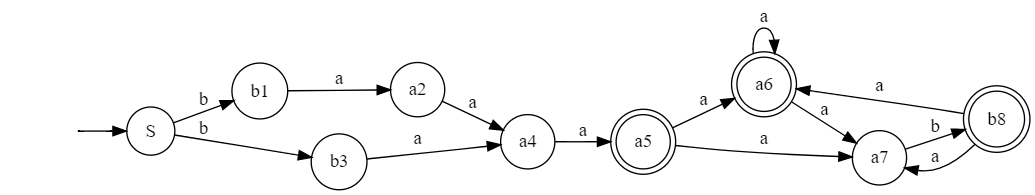
\includegraphics[width=4in, keepaspectratio]{glushkov1.png} % the Glushkov diagram placeholder

  Подграфы, распознающие регулярные выражения, являющиеся подструктурами исходного, не имеют общих вершин. Это свойство автомата Глушкова используется в реализациях \texttt{match}-функций некоторых библиотек регулярных выражений. %overall documentation
\end{frame}

% overall documentation : section 
\section{Обсуждение}
%В разделе "обсуждение" можно добавлять всё что угодно по вкусу: историческую справку, какие-то интересные примеры, способы применения, связь с другими понятиями теории автоматов и т.д. Можно сделать дополнительный метакомментарий: basic documentation, добавляющую ещё какие-то простые пояснения.
\begin{frame}{Cвойства автомата Глушкова}
  \begin{itemize}
    \item Не содержит $\empt$-переходов.
    \item Число состояний равно длине регулярного выражения (без учёта регулярных операций), плюс один (стартовое состояние).
    \item В общем случае недетерминированный.
  \end{itemize}

  \begin{alertblock}{\bf Примечание}
    Для $1$-однозначных регулярных выражений $r$ автомат $\Glushkov(r)$ является детерминированным. Эту его особенность активно используют в современных библиотеках регулярных выражений, например, в \textsc{RE2}. Выигрыш может получиться колоссальным: например, $\Thompson(\regexpstr(a\star)\star)$ является экспоненциально неоднозначным, а $\Glushkov(\regexpstr(a\star)\star)$ однозначен и детерминирован!
  \end{alertblock}% advanced documentation
\end{frame}
\end{document}
